% ========================================================
% FILE: sections/2.Database_Design.tex
% Chapter 2 of the sample Report 4: Database Design
%   intro + entity-relationship diagram
%   2.1 Table Relationships
%   "Table Descriptions" label + one row per table with
%   description, primary keys and foreign keys (sample format)
%   2.2 Module Entity--Relationship Diagrams (ERD1 .. ERD22)
% Primary and foreign keys are taken from apps/api/prisma/schema.prisma
% (@id, @@id and @relation(fields: [...])).
% ========================================================
\section{Database Design}

Frevia persists every domain object in a single PostgreSQL database whose schema is
declared with Prisma 7 in \texttt{apps/api/prisma/schema.prisma}. The schema contains
71 models together with 43 enumerations, every table has a surrogate integer primary
key generated by the database (nine membership tables use a composite key instead), and
deletion is either restricted by a foreign-key rule (identity and money-related rows are
never removed) or implemented as a soft delete through a \texttt{deletedAt} column
(content that an administrator must be able to restore: jobs, forum categories and posts,
skills, banners, contract term templates). Binary files are not stored in the database:
only their Cloudinary URL is kept in the owning row.

Figure~\ref{fig:db:erd} shows the entity--relationship diagram of the whole schema.
Every table is drawn as a frameless box: the header carries the table name, each of the
following rows is one column, and the key columns are flagged with \texttt{PK} (primary
key) or \texttt{FK} (foreign key). A relationship is a line that leaves the many-side
table with a crow's foot and ends on the one-side table with a single bar, so it reads
from the row that holds the foreign key to the row it references.

\begin{landscape}
\begin{figure}[p]
    \centering
    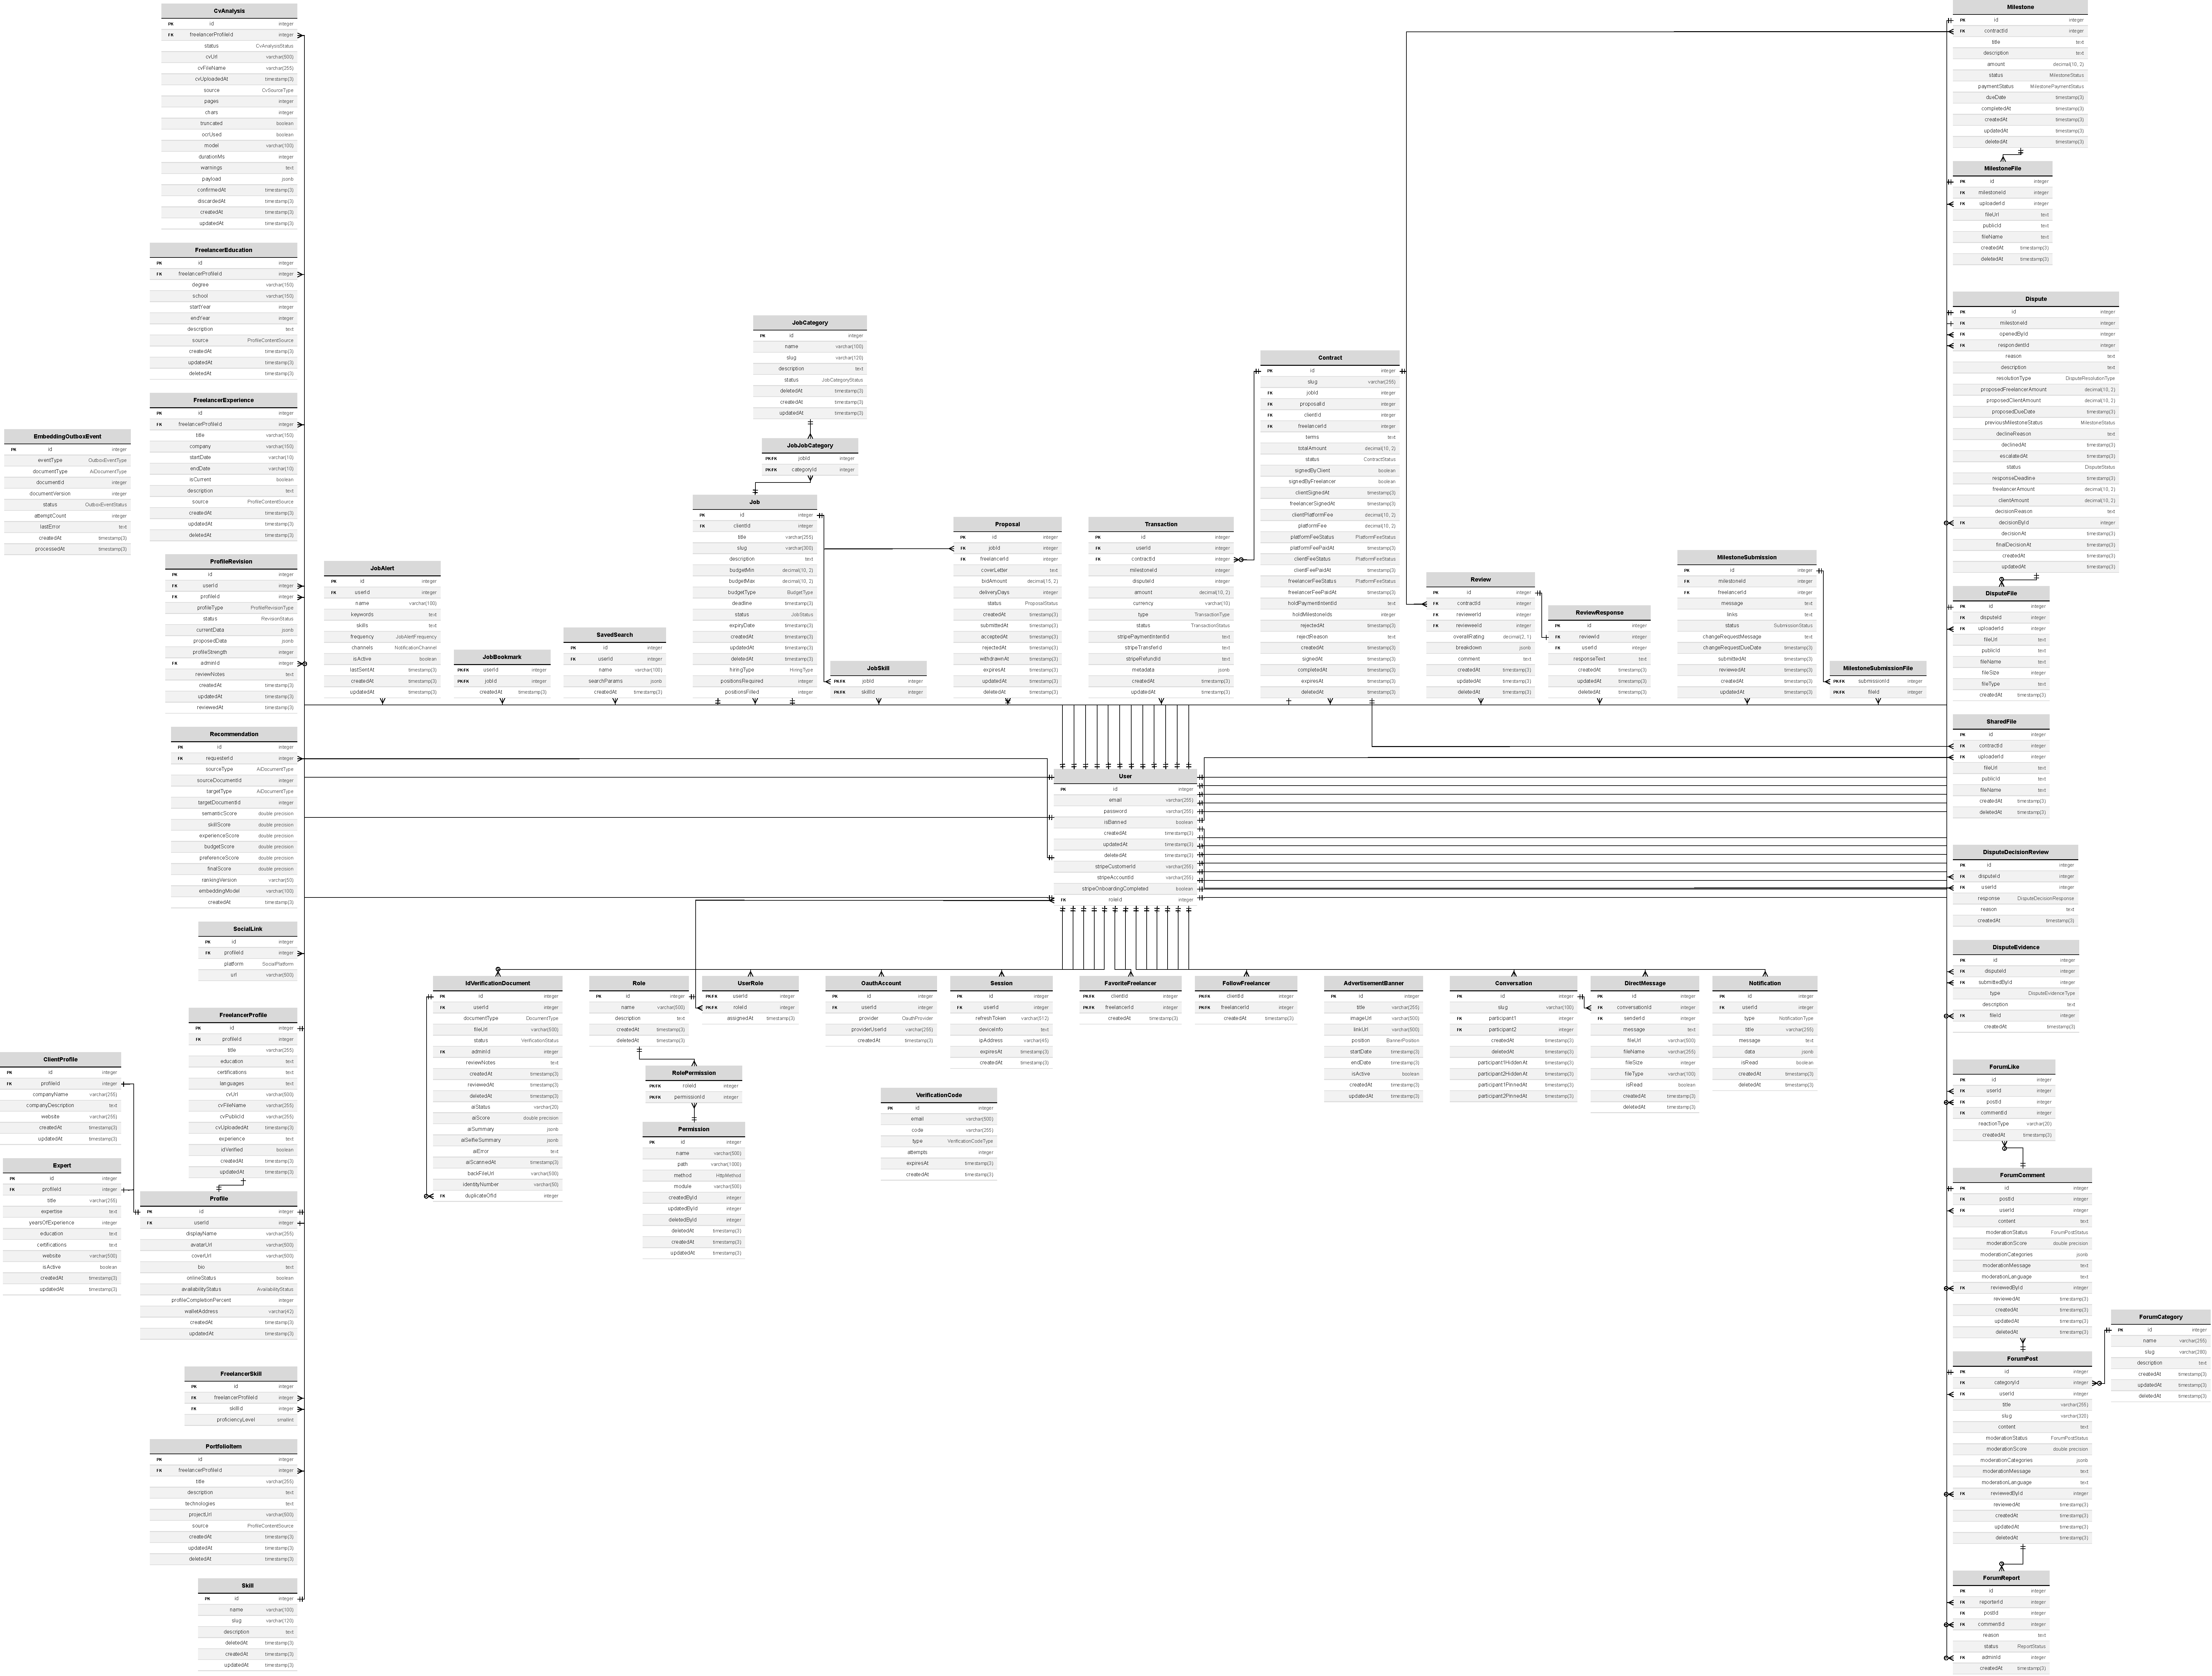
\includegraphics[width=0.98\linewidth,height=0.58\linewidth,keepaspectratio]{images/database/erd.pdf}
    \caption{Entity--relationship diagram of the Frevia database}
    \label{fig:db:erd}
\end{figure}
\end{landscape}

\subsection{Table Relationships}

The 71 tables are grouped into nine families; inside a family the relationships are
one-to-many, and membership tables carry the many-to-many links:

\begin{itemize}[leftmargin=*]\sloppy
    \item \textbf{Identity and access} --- \texttt{User} is the root of the schema and now also carries a required \texttt{roleId} that points to its primary \texttt{Role}; \texttt{UserRole} still links an account to any additional \texttt{Role}, and \texttt{RolePermission} links a role to a \texttt{Permission}, which yields the RBAC model enforced by the guards. Authentication adds \texttt{Session} (one row per device), \texttt{VerificationCode} (OTP for registration and password reset), \texttt{OauthAccount} (Google login), \texttt{TwoFactorAuth} and \texttt{UserSetting}.
    \item \textbf{Profiles} --- \texttt{Profile} is shared by every account; \texttt{FreelancerProfile} and \texttt{ClientProfile} extend it with role-specific columns, \texttt{Expert} publishes an expert entry in the public directory, and \texttt{FreelancerSkill} joins a freelancer to the \texttt{Skill} catalogue. \texttt{PortfolioItem}, \texttt{SocialLink}, \texttt{Certificate}, \texttt{IdVerificationDocument}, \texttt{ProfileRevision}, \texttt{CvAnalysis}, \texttt{FreelancerExperience} and \texttt{FreelancerEducation} hang from the profile. AI indexing and matching are tracked separately through \texttt{DocumentProcessingJob}, \texttt{EmbeddingIndexRecord}, \texttt{Recommendation} and \texttt{EmbeddingOutboxEvent}.
    \item \textbf{Jobs} --- \texttt{Job} belongs to a client and is classified through \texttt{JobJobCategory} (\texttt{JobCategory}) and \texttt{JobSkill} (\texttt{Skill}). \texttt{JobBookmark}, \texttt{RecentlyViewedJob}, \texttt{SavedSearch} and \texttt{JobAlert} record the browsing behaviour of a freelancer.
    \item \textbf{Proposals and contracts} --- \texttt{Proposal} references one \texttt{Job} and one freelancer; accepting it creates exactly one \texttt{Contract}, which carries \texttt{ContractTermTemplate} snapshots and a list of \texttt{Milestone} rows. \texttt{ProjectProgressUpdate}, \texttt{SharedFile} and \texttt{MilestoneFile} document the work in progress, while \texttt{MilestoneSubmission} (with \texttt{MilestoneSubmissionFile}) records the deliverable and its review decision.
    \item \textbf{Payments} --- \texttt{Transaction} stores every Stripe movement (funding, release, refund, platform fee, dispute fee) with its payment-intent identifier, and \texttt{Invoice} holds the invoice issued per contract. Money is never derived: the escrow balance of a milestone is the sum of its transactions.
    \item \textbf{Disputes} --- \texttt{Dispute} is opened on a contract or a milestone, \texttt{DisputeEvidence} collects the attachments of both parties, \texttt{DisputeFee} records the fee charged to open it, and \texttt{DisputeDecisionReview} stores the request of a party that asks for the decision to be reconsidered.
    \item \textbf{Reviews} --- one \texttt{Review} per completed contract, answered by at most one \texttt{ReviewResponse}.
    \item \textbf{Messaging and notifications} --- \texttt{Conversation} groups the \texttt{DirectMessage} rows exchanged by two accounts (pin and read state are kept on the message and on the conversation), and \texttt{Notification} feeds the in-app bell.
    \item \textbf{Community forum and configuration} --- \texttt{ForumCategory} contains \texttt{ForumPost}, a post contains \texttt{ForumComment}, and \texttt{ForumLike} / \texttt{ForumReport} attach reactions and reports to posts or comments. \texttt{ForumPost} and \texttt{ForumComment} may also store reviewer metadata for moderated content. Administrators manage reports through \texttt{ModerationQueue} (while \texttt{BannedKeyword} is reserved in the schema and currently unexposed by the API); platform-wide configuration lives in \texttt{SystemSetting}, \texttt{AnnouncementBanner} and \texttt{AdvertisementBanner}.
\end{itemize}

\subsubsection*{Table Descriptions}

Table~\ref{tab:db:tables} describes the purpose of every table of the schema, in the
order in which the models are declared in \texttt{schema.prisma}, together with its
primary key and its foreign keys.

{\small
\begin{longtable}{|C{0.9cm}|L{5.0cm}|L{8.8cm}|}
\caption{Table descriptions of the Frevia database}
\label{tab:db:tables}
\\
\hline
\rowcolor{headerbg}\textbf{No} & \textbf{Table} & \textbf{Description} \\ \hline
\endfirsthead
\hline
\rowcolor{headerbg}\textbf{No} & \textbf{Table} & \textbf{Description} \\ \hline
\endhead
\hline\endfoot
\hline\endlastfoot
\texttt{01} & \texttt{Role} & Role catalogue of the RBAC model (admin, client, freelancer, expert); carries the role code, name and description.
\newline \textbullet~\textbf{Primary keys:} \texttt{id}
\newline \textbullet~\textbf{Foreign keys:} --- \\ \hline
\texttt{02} & \texttt{UserRole} & Assignment of a role to an account, so one account can hold several roles and switch between them.
\newline \textbullet~\textbf{Primary keys:} \texttt{userId}, \texttt{roleId}
\newline \textbullet~\textbf{Foreign keys:} \texttt{userId} $\rightarrow$ \texttt{User}, \texttt{roleId} $\rightarrow$ \texttt{Role} \\ \hline
\texttt{03} & \texttt{Permission} & Catalogue of route-level permissions (\texttt{module.action} names) used by the permission guard.
\newline \textbullet~\textbf{Primary keys:} \texttt{id}
\newline \textbullet~\textbf{Foreign keys:} --- \\ \hline
\texttt{04} & \texttt{RolePermission} & Permissions granted to a role; drives the effective permission list of every signed-in account.
\newline \textbullet~\textbf{Primary keys:} \texttt{roleId}, \texttt{permissionId}
\newline \textbullet~\textbf{Foreign keys:} \texttt{roleId} $\rightarrow$ \texttt{Role}, \texttt{permissionId} $\rightarrow$ \texttt{Permission} \\ \hline
\texttt{05} & \texttt{User} & Account identity: e-mail, bcrypt password hash, ban flag, Stripe customer/Connect flags and timestamps. Carries the primary role through \texttt{roleId}.
\newline \textbullet~\textbf{Primary keys:} \texttt{id}
\newline \textbullet~\textbf{Foreign keys:} \texttt{roleId} $\rightarrow$ \texttt{Role} \\ \hline
\texttt{06} & \texttt{VerificationCode} & One-time code (OTP) issued for e-mail verification or password reset, with its purpose (\texttt{type}), verification attempt counter (\texttt{attempts}) and expiry; consumed codes are deleted.
\newline \textbullet~\textbf{Primary keys:} \texttt{id}
\newline \textbullet~\textbf{Foreign keys:} --- \\ \hline
\texttt{07} & \texttt{Session} & Server-side session per device: refresh-token hash, device/user-agent and IP address metadata, and expiry timestamp.
\newline \textbullet~\textbf{Primary keys:} \texttt{id}
\newline \textbullet~\textbf{Foreign keys:} \texttt{userId} $\rightarrow$ \texttt{User} \\ \hline
\texttt{08} & \texttt{OauthAccount} & Link between an account and an external identity provider (Google) for federated login.
\newline \textbullet~\textbf{Primary keys:} \texttt{id}
\newline \textbullet~\textbf{Foreign keys:} \texttt{userId} $\rightarrow$ \texttt{User} \\ \hline
\texttt{09} & \texttt{TwoFactorAuth} & Two-factor authentication secret and enabled flag of an account (one row per account).
\newline \textbullet~\textbf{Primary keys:} \texttt{id}
\newline \textbullet~\textbf{Foreign keys:} \texttt{userId} $\rightarrow$ \texttt{User} \\ \hline
\texttt{10} & \texttt{UserSetting} & Per-account preferences: interface theme, language and the JSON notification preferences.
\newline \textbullet~\textbf{Primary keys:} \texttt{id}
\newline \textbullet~\textbf{Foreign keys:} \texttt{userId} $\rightarrow$ \texttt{User} \\ \hline
\texttt{11} & \texttt{Profile} & Base profile shared by all accounts: display name, avatar, cover, biography, availability status and completion percentage.
\newline \textbullet~\textbf{Primary keys:} \texttt{id}
\newline \textbullet~\textbf{Foreign keys:} \texttt{userId} $\rightarrow$ \texttt{User} \\ \hline
\texttt{12} & \texttt{FreelancerProfile} & Professional data of a freelancer: professional title, education, certifications, languages, experience summaries, uploaded CV metadata and identity verification flag.
\newline \textbullet~\textbf{Primary keys:} \texttt{id}
\newline \textbullet~\textbf{Foreign keys:} \texttt{profileId} $\rightarrow$ \texttt{Profile} \\ \hline
\texttt{13} & \texttt{FreelancerSkill} & Many-to-many link between a freelancer profile and a skill, with the self-declared proficiency level.
\newline \textbullet~\textbf{Primary keys:} \texttt{id}
\newline \textbullet~\textbf{Foreign keys:} \texttt{freelancerProfileId} $\rightarrow$ \texttt{FreelancerProfile}, \texttt{skillId} $\rightarrow$ \texttt{Skill} \\ \hline
\texttt{14} & \texttt{ClientProfile} & Client-side data: company name, company description and website URL.
\newline \textbullet~\textbf{Primary keys:} \texttt{id}
\newline \textbullet~\textbf{Foreign keys:} \texttt{profileId} $\rightarrow$ \texttt{Profile} \\ \hline
\texttt{15} & \texttt{Expert} & Expert entry published in the public expert directory, with specialisation and verification state.
\newline \textbullet~\textbf{Primary keys:} \texttt{id}
\newline \textbullet~\textbf{Foreign keys:} \texttt{profileId} $\rightarrow$ \texttt{Profile} \\ \hline
\texttt{16} & \texttt{ProfileRevision} & Pending change request on a profile, reviewed and approved or rejected by an administrator.
\newline \textbullet~\textbf{Primary keys:} \texttt{id}
\newline \textbullet~\textbf{Foreign keys:} \texttt{userId} $\rightarrow$ \texttt{User}, \texttt{adminId} $\rightarrow$ \texttt{User}, \texttt{profileId} $\rightarrow$ \texttt{Profile} \\ \hline
\texttt{17} & \texttt{PortfolioItem} & Portfolio entry of a profile: title, description, technologies list, project URL, content source and soft-delete support.
\newline \textbullet~\textbf{Primary keys:} \texttt{id}
\newline \textbullet~\textbf{Foreign keys:} \texttt{freelancerProfileId} $\rightarrow$ \texttt{FreelancerProfile} \\ \hline
\texttt{18} & \texttt{CvAnalysis} & AI analysis of a freelancer CV: upload metadata, extraction statistics, the structured JSON result (skills, experience, education, projects, summary) and the confirmation state. Generating a new analysis discards any prior \texttt{PENDING} draft for the profile.
\newline \textbullet~\textbf{Primary keys:} \texttt{id}
\newline \textbullet~\textbf{Foreign keys:} \texttt{freelancerProfileId} $\rightarrow$ \texttt{FreelancerProfile} \\ \hline
\texttt{19} & \texttt{FreelancerExperience} & Experience item of a freelancer profile, either entered manually or imported from a CV, with company, dates and description.
\newline \textbullet~\textbf{Primary keys:} \texttt{id}
\newline \textbullet~\textbf{Foreign keys:} \texttt{freelancerProfileId} $\rightarrow$ \texttt{FreelancerProfile} \\ \hline
\texttt{20} & \texttt{FreelancerEducation} & Education item of a freelancer profile, either entered manually or imported from a CV, with degree, school and years.
\newline \textbullet~\textbf{Primary keys:} \texttt{id}
\newline \textbullet~\textbf{Foreign keys:} \texttt{freelancerProfileId} $\rightarrow$ \texttt{FreelancerProfile} \\ \hline
\texttt{21} & \texttt{DocumentProcessingJob} & Asynchronous processing job for an AI document (CV, job description, proposal): document type, document id, version, status, attempt counter and error message.
\newline \textbullet~\textbf{Primary keys:} \texttt{id}
\newline \textbullet~\textbf{Foreign keys:} --- \\ \hline
\texttt{22} & \texttt{EmbeddingIndexRecord} & Vector index record for a document section: embedding model, collection, vector record id, content hash and index status.
\newline \textbullet~\textbf{Primary keys:} \texttt{id}
\newline \textbullet~\textbf{Foreign keys:} --- \\ \hline
\texttt{23} & \texttt{Recommendation} & Job--CV recommendation result: requester, source and target document references, score breakdown (semantic, skill, experience, budget, preference), ranking version and embedding model.
\newline \textbullet~\textbf{Primary keys:} \texttt{id}
\newline \textbullet~\textbf{Foreign keys:} \texttt{requesterId} $\rightarrow$ \texttt{User} \\ \hline
\texttt{24} & \texttt{EmbeddingOutboxEvent} & Outbox event that triggers embedding or re-indexing of a document, with event type, document reference, status, attempt counter and processing timestamp.
\newline \textbullet~\textbf{Primary keys:} \texttt{id}
\newline \textbullet~\textbf{Foreign keys:} --- \\ \hline
\texttt{25} & \texttt{SocialLink} & External link of a profile (website, LinkedIn, GitHub, Behance) shown on the public profile.
\newline \textbullet~\textbf{Primary keys:} \texttt{id}
\newline \textbullet~\textbf{Foreign keys:} \texttt{profileId} $\rightarrow$ \texttt{Profile} \\ \hline
\texttt{26} & \texttt{IdVerificationDocument} & Identity document uploaded for eKYC, with the AI check result and the administrator decision.
\newline \textbullet~\textbf{Primary keys:} \texttt{id}
\newline \textbullet~\textbf{Foreign keys:} \texttt{userId} $\rightarrow$ \texttt{User}, \texttt{adminId} $\rightarrow$ \texttt{User}, \texttt{duplicateOfId} $\rightarrow$ \texttt{IdVerificationDocument} \\ \hline
\texttt{27} & \texttt{ProfileVisitLog} & View log of a freelancer profile (\texttt{viewerId}, \texttt{targetFreelancerId}, \texttt{viewedAt}); source of the profile statistics.
\newline \textbullet~\textbf{Primary keys:} \texttt{id}
\newline \textbullet~\textbf{Foreign keys:} \texttt{viewerId} $\rightarrow$ \texttt{User}, \texttt{targetFreelancerId} $\rightarrow$ \texttt{User} \\ \hline
\texttt{28} & \texttt{JobCategory} & Flat job category (\texttt{name}, \texttt{slug}, \texttt{description}, \texttt{status}) with soft-delete support.
\newline \textbullet~\textbf{Primary keys:} \texttt{id}
\newline \textbullet~\textbf{Foreign keys:} --- \\ \hline
\texttt{29} & \texttt{Job} & Job posting: slug, title, description, budget range and type, hiring type, positions required/filled, deadline, expiry date, status and the owning client.
\newline \textbullet~\textbf{Primary keys:} \texttt{id}
\newline \textbullet~\textbf{Foreign keys:} \texttt{clientId} $\rightarrow$ \texttt{User} \\ \hline
\texttt{30} & \texttt{JobJobCategory} & Many-to-many link between a job and the job categories it is published in.
\newline \textbullet~\textbf{Primary keys:} \texttt{jobId}, \texttt{categoryId}
\newline \textbullet~\textbf{Foreign keys:} \texttt{jobId} $\rightarrow$ \texttt{Job}, \texttt{categoryId} $\rightarrow$ \texttt{JobCategory} \\ \hline
\texttt{31} & \texttt{Skill} & Skill catalogue shared by freelancer profiles and jobs, with soft-delete support.
\newline \textbullet~\textbf{Primary keys:} \texttt{id}
\newline \textbullet~\textbf{Foreign keys:} --- \\ \hline
\texttt{32} & \texttt{JobSkill} & Many-to-many link pairing a job with its required skills.
\newline \textbullet~\textbf{Primary keys:} \texttt{jobId}, \texttt{skillId}
\newline \textbullet~\textbf{Foreign keys:} \texttt{jobId} $\rightarrow$ \texttt{Job}, \texttt{skillId} $\rightarrow$ \texttt{Skill} \\ \hline
\texttt{33} & \texttt{JobBookmark} & Jobs saved by a freelancer.
\newline \textbullet~\textbf{Primary keys:} \texttt{userId}, \texttt{jobId}
\newline \textbullet~\textbf{Foreign keys:} \texttt{userId} $\rightarrow$ \texttt{User}, \texttt{jobId} $\rightarrow$ \texttt{Job} \\ \hline
\texttt{34} & \texttt{RecentlyViewedJob} & Recently opened job postings of an account, with the viewing timestamp.
\newline \textbullet~\textbf{Primary keys:} \texttt{id}
\newline \textbullet~\textbf{Foreign keys:} \texttt{userId} $\rightarrow$ \texttt{User}, \texttt{jobId} $\rightarrow$ \texttt{Job} \\ \hline
\texttt{35} & \texttt{SavedSearch} & Stored job filter criteria (keyword, categories, budget, skills) that the freelancer can reapply.
\newline \textbullet~\textbf{Primary keys:} \texttt{id}
\newline \textbullet~\textbf{Foreign keys:} \texttt{userId} $\rightarrow$ \texttt{User} \\ \hline
\texttt{36} & \texttt{JobAlert} & User-level job alert configuration storing keywords, skills, frequency, notification channels and active flag.
\newline \textbullet~\textbf{Primary keys:} \texttt{id}
\newline \textbullet~\textbf{Foreign keys:} \texttt{userId} $\rightarrow$ \texttt{User} \\ \hline
\texttt{37} & \texttt{Proposal} & Proposal submitted by a freelancer for a job: cover letter, bid amount, estimated duration and lifecycle status.
\newline \textbullet~\textbf{Primary keys:} \texttt{id}
\newline \textbullet~\textbf{Foreign keys:} \texttt{jobId} $\rightarrow$ \texttt{Job}, \texttt{freelancerId} $\rightarrow$ \texttt{User} \\ \hline
\texttt{38} & \texttt{ProposalAttachment} & File attached to a proposal (portfolio sample, reference document) stored in Cloudinary.
\newline \textbullet~\textbf{Primary keys:} \texttt{id}
\newline \textbullet~\textbf{Foreign keys:} \texttt{proposalId} $\rightarrow$ \texttt{Proposal} \\ \hline
\texttt{39} & \texttt{Contract} & Contract created when a proposal is accepted: slug, client, freelancer, total amount, terms, bilateral signature flags/timestamps, platform fee fields, Stripe hold reference, expiry/completion dates and status.
\newline \textbullet~\textbf{Primary keys:} \texttt{id}
\newline \textbullet~\textbf{Foreign keys:} \texttt{jobId} $\rightarrow$ \texttt{Job}, \texttt{proposalId} $\rightarrow$ \texttt{Proposal}, \texttt{clientId} $\rightarrow$ \texttt{User}, \texttt{freelancerId} $\rightarrow$ \texttt{User} \\ \hline
\texttt{40} & \texttt{ContractTermTemplate} & Reusable contract term template owned by a user, with category, content and soft-delete support.
\newline \textbullet~\textbf{Primary keys:} \texttt{id}
\newline \textbullet~\textbf{Foreign keys:} \texttt{creatorId} $\rightarrow$ \texttt{User} \\ \hline
\texttt{41} & \texttt{Milestone} & Milestone inside a contract: title, description, amount, due date, completion date, milestone lifecycle status and payment escrow status.
\newline \textbullet~\textbf{Primary keys:} \texttt{id}
\newline \textbullet~\textbf{Foreign keys:} \texttt{contractId} $\rightarrow$ \texttt{Contract} \\ \hline
\texttt{42} & \texttt{MilestoneFile} & Reference file attached to a milestone and shared with both parties.
\newline \textbullet~\textbf{Primary keys:} \texttt{id}
\newline \textbullet~\textbf{Foreign keys:} \texttt{milestoneId} $\rightarrow$ \texttt{Milestone}, \texttt{uploaderId} $\rightarrow$ \texttt{User} \\ \hline
\texttt{43} & \texttt{MilestoneSubmission} & Work submitted for a milestone, with the submitted note, timestamp and the client review decision.
\newline \textbullet~\textbf{Primary keys:} \texttt{id}
\newline \textbullet~\textbf{Foreign keys:} \texttt{milestoneId} $\rightarrow$ \texttt{Milestone}, \texttt{freelancerId} $\rightarrow$ \texttt{User} \\ \hline
\texttt{44} & \texttt{MilestoneSubmissionFile} & Join table linking a submission to the milestone files it delivers.
\newline \textbullet~\textbf{Primary keys:} \texttt{submissionId}, \texttt{fileId}
\newline \textbullet~\textbf{Foreign keys:} \texttt{submissionId} $\rightarrow$ \texttt{MilestoneSubmission}, \texttt{fileId} $\rightarrow$ \texttt{MilestoneFile} \\ \hline
\texttt{45} & \texttt{Invoice} & Invoice of a contract (one per contract): invoice number, total amount, status, issued, due and paid dates.
\newline \textbullet~\textbf{Primary keys:} \texttt{id}
\newline \textbullet~\textbf{Foreign keys:} \texttt{contractId} $\rightarrow$ \texttt{Contract} \\ \hline
\texttt{46} & \texttt{Certificate} & Completion certificate generated when a contract is finished: unique certificate UID, completion date and JSON metadata.
\newline \textbullet~\textbf{Primary keys:} \texttt{id}
\newline \textbullet~\textbf{Foreign keys:} \texttt{contractId} $\rightarrow$ \texttt{Contract}, \texttt{freelancerId} $\rightarrow$ \texttt{User}, \texttt{clientId} $\rightarrow$ \texttt{User} \\ \hline
\texttt{47} & \texttt{Dispute} & Dispute opened on a contract or a milestone: reason, description, opened by, status, resolution and decision timestamps.
\newline \textbullet~\textbf{Primary keys:} \texttt{id}
\newline \textbullet~\textbf{Foreign keys:} \texttt{milestoneId} $\rightarrow$ \texttt{Milestone}, \texttt{openedById} $\rightarrow$ \texttt{User}, \texttt{respondentId} $\rightarrow$ \texttt{User}, \texttt{decisionById} $\rightarrow$ \texttt{User} \\ \hline
\texttt{48} & \texttt{DisputeFee} & Fee charged to open a dispute, with its amount, payment state and the transaction that settled it.
\newline \textbullet~\textbf{Primary keys:} \texttt{id}
\newline \textbullet~\textbf{Foreign keys:} \texttt{disputeId} $\rightarrow$ \texttt{Dispute}, \texttt{userId} $\rightarrow$ \texttt{User} \\ \hline
\texttt{49} & \texttt{DisputeEvidence} & Evidence attached by either party to a dispute (file, description, uploader).
\newline \textbullet~\textbf{Primary keys:} \texttt{id}
\newline \textbullet~\textbf{Foreign keys:} \texttt{disputeId} $\rightarrow$ \texttt{Dispute}, \texttt{submittedById} $\rightarrow$ \texttt{User}, \texttt{fileId} $\rightarrow$ \texttt{SharedFile} \\ \hline
\texttt{50} & \texttt{DisputeDecisionReview} & Request of a party to reconsider a dispute decision, with the response, the reason and the timestamp.
\newline \textbullet~\textbf{Primary keys:} \texttt{id}
\newline \textbullet~\textbf{Foreign keys:} \texttt{disputeId} $\rightarrow$ \texttt{Dispute}, \texttt{userId} $\rightarrow$ \texttt{User} \\ \hline
\texttt{51} & \texttt{Transaction} & Payment movement reconciled with Stripe (funding, release, refund, platform fee, dispute fee): type, amount, status, payment-intent id and timestamps.
\newline \textbullet~\textbf{Primary keys:} \texttt{id}
\newline \textbullet~\textbf{Foreign keys:} \texttt{userId} $\rightarrow$ \texttt{User}, \texttt{contractId} $\rightarrow$ \texttt{Contract} \\ \hline
\texttt{52} & \texttt{Review} & Review written after a contract is completed: rating, comment, author, recipient and the reviewed contract.
\newline \textbullet~\textbf{Primary keys:} \texttt{id}
\newline \textbullet~\textbf{Foreign keys:} \texttt{contractId} $\rightarrow$ \texttt{Contract}, \texttt{reviewerId} $\rightarrow$ \texttt{User}, \texttt{revieweeId} $\rightarrow$ \texttt{User} \\ \hline
\texttt{53} & \texttt{ReviewResponse} & Reply of the reviewed party to a review (at most one per review).
\newline \textbullet~\textbf{Primary keys:} \texttt{id}
\newline \textbullet~\textbf{Foreign keys:} \texttt{reviewId} $\rightarrow$ \texttt{Review}, \texttt{userId} $\rightarrow$ \texttt{User} \\ \hline
\texttt{54} & \texttt{ForumCategory} & Forum category: slug, name, description and soft-delete support.
\newline \textbullet~\textbf{Primary keys:} \texttt{id}
\newline \textbullet~\textbf{Foreign keys:} --- \\ \hline
\texttt{55} & \texttt{ForumPost} & Forum post: title, content, author, category, moderation status, AI score, reviewer and soft-delete support.
\newline \textbullet~\textbf{Primary keys:} \texttt{id}
\newline \textbullet~\textbf{Foreign keys:} \texttt{categoryId} $\rightarrow$ \texttt{ForumCategory}, \texttt{userId} $\rightarrow$ \texttt{User}, \texttt{reviewedById} $\rightarrow$ \texttt{User} \\ \hline
\texttt{56} & \texttt{ForumComment} & Comment on a forum post; comments are one level deep and can be soft-deleted. Review metadata is stored when an administrator moderates the comment.
\newline \textbullet~\textbf{Primary keys:} \texttt{id}
\newline \textbullet~\textbf{Foreign keys:} \texttt{postId} $\rightarrow$ \texttt{ForumPost}, \texttt{userId} $\rightarrow$ \texttt{User}, \texttt{reviewedById} $\rightarrow$ \texttt{User} \\ \hline
\texttt{57} & \texttt{ForumLike} & Reaction of a member on a post or a comment; a member can like a target only once.
\newline \textbullet~\textbf{Primary keys:} \texttt{id}
\newline \textbullet~\textbf{Foreign keys:} \texttt{userId} $\rightarrow$ \texttt{User}, \texttt{postId} $\rightarrow$ \texttt{ForumPost}, \texttt{commentId} $\rightarrow$ \texttt{ForumComment} \\ \hline
\texttt{58} & \texttt{ForumReport} & Content report filed by a member: reason, status and the administrator who handled it.
\newline \textbullet~\textbf{Primary keys:} \texttt{id}
\newline \textbullet~\textbf{Foreign keys:} \texttt{reporterId} $\rightarrow$ \texttt{User}, \texttt{postId} $\rightarrow$ \texttt{ForumPost}, \texttt{commentId} $\rightarrow$ \texttt{ForumComment}, \texttt{adminId} $\rightarrow$ \texttt{User} \\ \hline
\texttt{59} & \texttt{Notification} & In-app notification of an account: type, title, body, target link and read state.
\newline \textbullet~\textbf{Primary keys:} \texttt{id}
\newline \textbullet~\textbf{Foreign keys:} \texttt{userId} $\rightarrow$ \texttt{User} \\ \hline
\texttt{60} & \texttt{AnnouncementBanner} & Platform announcement shown in the application: message, link, display window, active flag and soft delete.
\newline \textbullet~\textbf{Primary keys:} \texttt{id}
\newline \textbullet~\textbf{Foreign keys:} --- \\ \hline
\texttt{61} & \texttt{ModerationQueue} & Queue of AI-flagged or user-reported content waiting for an administrator decision, with the item type (\texttt{contentType}), target identifier, reason, status, handling administrator and action taken.
\newline \textbullet~\textbf{Primary keys:} \texttt{id}
\newline \textbullet~\textbf{Foreign keys:} \texttt{reporterId} $\rightarrow$ \texttt{User}, \texttt{adminId} $\rightarrow$ \texttt{User} \\ \hline
\texttt{62} & \texttt{SystemSetting} & Platform-wide configuration values stored as key/value rows.
\newline \textbullet~\textbf{Primary keys:} \texttt{id}
\newline \textbullet~\textbf{Foreign keys:} --- \\ \hline
\texttt{63} & \texttt{BannedKeyword} & Reserved keyword table in the schema, currently unexposed by the application API.
\newline \textbullet~\textbf{Primary keys:} \texttt{id}
\newline \textbullet~\textbf{Foreign keys:} \texttt{createdBy} $\rightarrow$ \texttt{User} \\ \hline
\texttt{64} & \texttt{AdvertisementBanner} & Advertising banner with title, image URL, target URL, position, schedule and active flag.
\newline \textbullet~\textbf{Primary keys:} \texttt{id}
\newline \textbullet~\textbf{Foreign keys:} --- \\ \hline
\texttt{65} & \texttt{FavoriteFreelancer} & Freelancers marked as favourite by a client account.
\newline \textbullet~\textbf{Primary keys:} \texttt{clientId}, \texttt{freelancerId}
\newline \textbullet~\textbf{Foreign keys:} \texttt{clientId} $\rightarrow$ \texttt{User}, \texttt{freelancerId} $\rightarrow$ \texttt{User} \\ \hline
\texttt{66} & \texttt{FollowFreelancer} & Follow relationship between two accounts, used by the activity feed.
\newline \textbullet~\textbf{Primary keys:} \texttt{clientId}, \texttt{freelancerId}
\newline \textbullet~\textbf{Foreign keys:} \texttt{clientId} $\rightarrow$ \texttt{User}, \texttt{freelancerId} $\rightarrow$ \texttt{User} \\ \hline
\texttt{67} & \texttt{PortfolioLike} & Like given on a portfolio item.
\newline \textbullet~\textbf{Primary keys:} \texttt{userId}, \texttt{portfolioItemId}
\newline \textbullet~\textbf{Foreign keys:} \texttt{userId} $\rightarrow$ \texttt{User}, \texttt{portfolioItemId} $\rightarrow$ \texttt{PortfolioItem} \\ \hline
\texttt{68} & \texttt{ProjectProgressUpdate} & Progress note posted by the freelancer on a contract, with the update timestamp.
\newline \textbullet~\textbf{Primary keys:} \texttt{id}
\newline \textbullet~\textbf{Foreign keys:} \texttt{contractId} $\rightarrow$ \texttt{Contract}, \texttt{freelancerId} $\rightarrow$ \texttt{User} \\ \hline
\texttt{69} & \texttt{SharedFile} & File shared in the workspace of a contract (both parties can upload and read).
\newline \textbullet~\textbf{Primary keys:} \texttt{id}
\newline \textbullet~\textbf{Foreign keys:} \texttt{contractId} $\rightarrow$ \texttt{Contract}, \texttt{uploaderId} $\rightarrow$ \texttt{User} \\ \hline
\texttt{70} & \texttt{Conversation} & Direct conversation between two accounts, storing per-participant hide/pin timestamps and soft-delete support.
\newline \textbullet~\textbf{Primary keys:} \texttt{id}
\newline \textbullet~\textbf{Foreign keys:} \texttt{participant1} $\rightarrow$ \texttt{User}, \texttt{participant2} $\rightarrow$ \texttt{User} \\ \hline
\texttt{71} & \texttt{DirectMessage} & Message of a conversation: sender, content, attachments, read state, recall (soft delete) flag and timestamp.
\newline \textbullet~\textbf{Primary keys:} \texttt{id}
\newline \textbullet~\textbf{Foreign keys:} \texttt{conversationId} $\rightarrow$ \texttt{Conversation}, \texttt{senderId} $\rightarrow$ \texttt{User} \\ \hline
\end{longtable}
}

% ========================================================
% 2.2 Module entity-relationship diagrams
% One figure per functional module of Report 3 (ERD1 .. ERD22).
% Source: database_design/ERD-ERD<n>.drawio
%         -> images/database/erd-<nn>.svg -> erd-<nn>.pdf (tools/svg2pdf.js)
% ========================================================
\subsection{Module Entity--Relationship Diagrams}
\label{sec:db:module-erds}

\subsubsection{ERD1 --- Authentication \& Sessions}

This ERD describes the Authentication \& Sessions module. It stores account identities, one-time verification codes, device sessions, OAuth links, two-factor authentication settings, and user preferences. User is the root account table and links to Role and Profile. VerificationCode supports registration, email verification, and password reset. Session stores refresh tokens and device information for each login. OauthAccount links Google login to a User. TwoFactorAuth stores the TOTP secret and enabled flag. UserSetting stores theme, language, and notification preferences. These tables support registration, login, logout, password reset, session revocation, Google OAuth, and 2FA.

\kfig{0.95\textwidth}{images/database/erd-01}{ERD1 --- Authentication \& Sessions}{fig:db:erd1}

\subsubsection{ERD2 --- Role-Based Access Control}

This ERD describes the Role-Based Access Control module. It stores roles, permissions, role-permission assignments, and user-role assignments. Role defines a named role; Permission defines a route-level permission; RolePermission links permissions to roles; UserRole links users to roles. These tables support RBAC guards, permission checks, and role switching without redeployment.

\kfig{0.95\textwidth}{images/database/erd-02}{ERD2 --- Role-Based Access Control}{fig:db:erd2}

\subsubsection{ERD3 --- Profile Core}

This ERD describes the Profile Core module. It stores base profiles and role-specific profile extensions. Profile contains common display information; FreelancerProfile stores professional data; ClientProfile stores company data; Expert publishes expert directory entries; FreelancerSkill links freelancers to skills with proficiency. These tables support profile viewing/editing, freelancer/client/expert profiles, skills, and profile completion.

\kfig{0.95\textwidth}{images/database/erd-03}{ERD3 --- Profile Core}{fig:db:erd3}

\subsubsection{ERD4 --- Profile History \& Social Links}

This ERD describes the Profile History \& Social Links module. It stores profile revisions, portfolio items, CV analysis, experience, education, document processing jobs, embedding records, recommendations, embedding outbox events, social links, identity documents, and profile visit logs. The CV-analysis and embedding tables were added to support AI CV processing, vector indexing and job--CV recommendation; they are linked to \texttt{FreelancerProfile} or \texttt{User} and do not change the existing profile-revision and social-link relationships. These tables support profile revision review, portfolio, CV processing, recommendations, social links, identity verification, and profile visit tracking.

\kfig{0.95\textwidth}{images/database/erd-04}{ERD4 --- Profile History \& Social Links}{fig:db:erd4}

\subsubsection{ERD5 --- Identity Verification \& Profile Visits}

This ERD describes the Identity Verification \& Profile Visits module. It stores identity verification documents and profile visit logs. These tables support eKYC document upload/review and tracking profile views.

\kfig{0.95\textwidth}{images/database/erd-05}{ERD5 --- Identity Verification \& Profile Visits}{fig:db:erd5}

\subsubsection{ERD6 --- Portfolio \& Skills}

This ERD describes the Portfolio \& Skills module. It stores portfolio items, freelancer skills, skill catalog, and portfolio likes. These tables support portfolio management, skill catalog, skill proficiency, and liking portfolios.

\kfig{0.95\textwidth}{images/database/erd-06}{ERD6 --- Portfolio \& Skills}{fig:db:erd6}

\subsubsection{ERD7 --- Favorites \& Follows}

This ERD describes the Favorites \& Follows module. It stores favorite freelancer and follow relationships. These tables support bookmarking favorite freelancers and managing follow relationships.

\kfig{0.95\textwidth}{images/database/erd-07}{ERD7 --- Favorites \& Follows}{fig:db:erd7}

\subsubsection{ERD8 --- Job Posting}

This ERD describes the Job Posting module. It stores job categories, jobs, job-category links, and job-skill links. These tables support creating, editing, publishing, closing, and categorizing jobs.

\kfig{0.95\textwidth}{images/database/erd-08}{ERD8 --- Job Posting}{fig:db:erd8}

\subsubsection{ERD9 --- Job Discovery \& Alerts}

This ERD describes the Job Discovery \& Alerts module. It stores job bookmarks, recently viewed jobs, saved searches, and job alerts. These tables support browsing, bookmarking, saved filters, and alert notifications.

\kfig{0.95\textwidth}{images/database/erd-09}{ERD9 --- Job Discovery \& Alerts}{fig:db:erd9}

\subsubsection{ERD10 --- Proposal}

This ERD describes the Proposal module. It stores proposals and proposal attachments. These tables support submitting, updating, withdrawing, accepting, and rejecting proposals.

\kfig{0.95\textwidth}{images/database/erd-10}{ERD10 --- Proposal}{fig:db:erd10}

\subsubsection{ERD11 --- Contract}

This ERD describes the Contract module. It stores contracts and contract term templates. These tables support contract creation, signing, cancellation, terms, and status management.

\kfig{0.95\textwidth}{images/database/erd-11}{ERD11 --- Contract}{fig:db:erd11}

\subsubsection{ERD12 --- Milestone \& Project Progress}

This ERD describes the Milestone \& Project Progress module. It stores milestones and project progress updates. These tables support milestone creation, updates, progress tracking, and client/freelancer collaboration.

\kfig{0.95\textwidth}{images/database/erd-12}{ERD12 --- Milestone \& Project Progress}{fig:db:erd12}

\subsubsection{ERD13 --- Milestone Submission}

This ERD describes the Milestone Submission module. It stores milestone files, submissions, and submission files. These tables support uploading deliverables, submitting milestones, and reviewing submissions.

\kfig{0.95\textwidth}{images/database/erd-13}{ERD13 --- Milestone Submission}{fig:db:erd13}

\subsubsection{ERD14 --- Escrow, Payments \& Certificates}

This ERD describes the Escrow, Payments \& Certificates module. It stores invoices, certificates, and transactions. These tables support funding, releasing, refunding, platform fees, payout tracking, and completion certificates.

\kfig{0.95\textwidth}{images/database/erd-14}{ERD14 --- Escrow, Payments \& Certificates}{fig:db:erd14}

\subsubsection{ERD15 --- Dispute Core}

This ERD describes the Dispute Core module. It stores disputes and dispute fees. These tables support opening disputes and charging dispute fees.

\kfig{0.95\textwidth}{images/database/erd-15}{ERD15 --- Dispute Core}{fig:db:erd15}

\subsubsection{ERD16 --- Dispute Resolution}

This ERD describes the Dispute Resolution module. It stores dispute evidence and decision reviews. These tables support evidence submission and review of dispute decisions.

\kfig{0.95\textwidth}{images/database/erd-16}{ERD16 --- Dispute Resolution}{fig:db:erd16}

\subsubsection{ERD17 --- Reviews \& Reputation}

This ERD describes the Reviews \& Reputation module. It stores reviews and review responses. These tables support rating contracts and responding to reviews.

\kfig{0.95\textwidth}{images/database/erd-17}{ERD17 --- Reviews \& Reputation}{fig:db:erd17}

\subsubsection{ERD18 --- Forum Posts \& Comments}

This ERD describes the Forum Posts \& Comments module. It stores forum categories, posts, and comments. These tables support forum discussions and moderation.

\kfig{0.95\textwidth}{images/database/erd-18}{ERD18 --- Forum Posts \& Comments}{fig:db:erd18}

\subsubsection{ERD19 --- Forum Likes}

This ERD describes the Forum Likes module. It stores likes on posts and comments. These tables support reactions.

\kfig{0.95\textwidth}{images/database/erd-19}{ERD19 --- Forum Likes}{fig:db:erd19}

\subsubsection{ERD20 --- Forum Reports \& Moderation}

This ERD describes the Forum Reports \& Moderation module. It stores forum reports, moderation queue, and banned keywords. These tables support reporting content and admin moderation.

\kfig{0.95\textwidth}{images/database/erd-20}{ERD20 --- Forum Reports \& Moderation}{fig:db:erd20}

\subsubsection{ERD21 --- Messaging \& Notifications}

This ERD describes the Messaging \& Notifications module. It stores notifications, conversations, and direct messages. These tables support real-time chat and in-app notifications.

\kfig{0.95\textwidth}{images/database/erd-21}{ERD21 --- Messaging \& Notifications}{fig:db:erd21}

\subsubsection{ERD22 --- Administration \& System}

This ERD describes the Administration \& System module. It stores announcement banners, system settings, and advertisement banners. These tables support admin configuration and banners.

\kfig{0.95\textwidth}{images/database/erd-22}{ERD22 --- Administration \& System}{fig:db:erd22}